\begin{figure}[h]
    \centering
    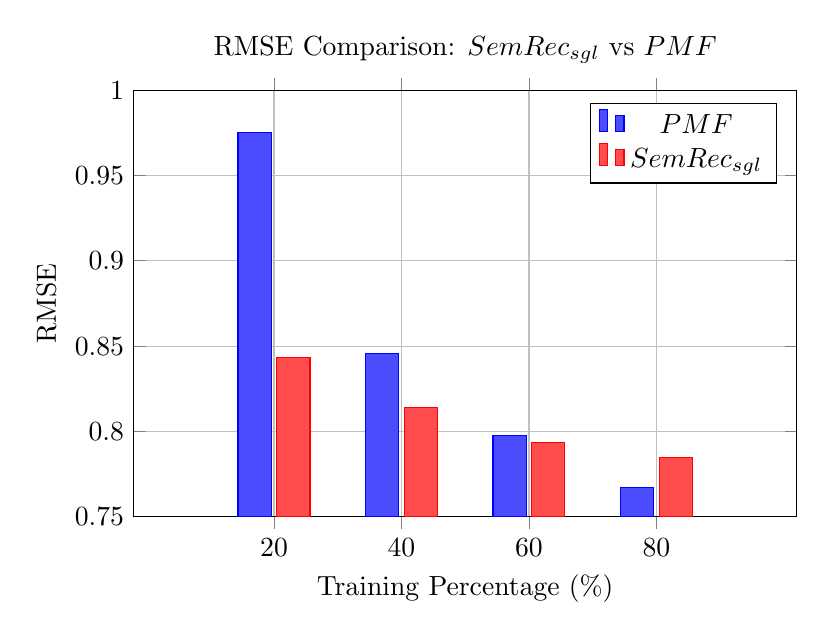
\begin{tikzpicture}
        \begin{axis}[
            xlabel={Training Percentage (\%)},
            ylabel={RMSE},
            title={RMSE Comparison: $SemRec_{sgl}$ vs $PMF$},
            ybar,
            bar width=12pt,
            grid=major,
            width=10cm,  % Reduced from 12cm
            height=7cm,  % Reduced from 8cm
            xmin=10, xmax=90,
            ymin=0.75, ymax=1.0,
            xtick={20,40,60,80},
            enlarge x limits=0.15,
            legend pos=north east,
        ]
        \addplot[fill=blue!70, draw=blue] coordinates {
            (20, 0.9750)
            (40, 0.8455)
            (60, 0.7975)
            (80, 0.7673)
        };
        \addplot[fill=red!70, draw=red] coordinates {
            (20, 0.8434)
            (40, 0.8138)
            (60, 0.7937)
            (80, 0.7846)
        };
        \legend{$PMF$, $SemRec_{sgl}$}
        \end{axis}
    \end{tikzpicture}
    \caption{Performance of $SemRec_{sgl}$ algorithm showing RMSE values across different training data percentages. SemRec is compared to positive matrix factorization. X-axis has the percentage of data used from database and y-axis has the RMSE of the method. Model trained on the Douban Data from article \parencite{shi2015semantic}.}
    \label{fig:semrec-rmse}
\end{figure}